\documentclass{homework}

\input{particulars}

\sisetup{round-precision=3}

\renewcommand\thesubsection{\arabic{subsection}}
\renewcommand\thesubsubsection{\thesubsection.\arabic{subsubsection}}

\begin{document}

\title{Machine Learning Homework \#6}
\author{\chineseName \masterStudentID}
\date{}
\maketitle

\subsection{Code}

All the code below is written in main.ipynb.

The imported modules are:

\begin{lstlisting}[language=Python]
import numpy as np
from scipy.spatial.distance import cdist
from PIL import Image
from IPython.display import display, Image as IPImage
from matplotlib import pyplot as plt
import cv2
import os
import time
\end{lstlisting}

Here is some helper function for adding coordinates features, execution time logging, save and show gif in Jupyter Notebook.

\begin{lstlisting}[language=Python]
def add_xy_coords(img):
    h, w, _ = img.shape
    
    x_coords = np.tile(np.arange(w), (h, 1))
    y_coords = np.tile(np.arange(h), (w, 1)).T
    new_img = np.concatenate((img, x_coords[:, :, np.newaxis], y_coords[:, :, np.newaxis]), axis=-1)

    return new_img

def log_execution_time(func):
    def wrapper(*args, **kwargs):
        start_time = time.time()
        result = func(*args, **kwargs)
        log_file = "execution_time.log"
        with open(log_file, "a") as f:
            f.write(
                f"{func.__name__}{kwargs} "
                f"{time.time() - start_time:.2f} s\n"
            )
        return result
    return wrapper

# history contains all previous labels for each pixel
# This will also save last frame to png
def save_history_to_gif(history, image_shape, filename, scale_factor=2):
    assert history.max() < 20, "We Don't support more than 20 clusters cmap :D"
    cmap = plt.get_cmap("tab20")
    image_history = history.reshape(-1, *image_shape)
    normalized_history = image_history / 20
    frames: list[Image.Image] = []
    for i in range(normalized_history.shape[0]):
        rgb_array = (cmap(normalized_history[i])[:, :, :3] * 255).astype(np.uint8)
        frame = Image.fromarray(rgb_array, mode="RGB")
        upscaled_frame = frame.resize(
            (image_shape[1] * scale_factor, image_shape[0] * scale_factor),
            resample=Image.NEAREST,
        )
        frames.append(upscaled_frame)

    frames[0].save(
        filename + ".gif",
        save_all=True,
        append_images=frames[1:],
        loop=0,
        duration=[100] * (len(frames) - 1) + [2000],
    )
    frames[-1].save(filename + ".png")

def display_gif(gif_filename):
    with open(gif_filename, "rb") as file:
        display(IPImage(file.read()))
\end{lstlisting}

The following code read the images and convert to proper format.

\begin{lstlisting}[language=Python]
images = [cv2.imread(f"image{i}.png") for i in [1, 2]]
images_rgb = [cv2.cvtColor(image, cv2.COLOR_BGR2RGB) for image in images]
images_xy = [add_xy_coords(image) for image in images_rgb]
print(images_xy[0].shape)
fig, ax = plt.subplots(1, len(images_rgb))
for i, image in enumerate(images_rgb):
    ax[i].imshow(image)
    ax[i].axis("off")
plt.tight_layout()
\end{lstlisting}

\subsubsection{Part 1 (Algorithm Implementation)}

The following code defines the new kernel, which follows the formula describe in spec.

\begin{lstlisting}[language=Python]
def compute_similarity_matrix(X, gamma_spatial=1.0, gamma_color=1.0):
    """
    Compute the similarity matrix using a Gaussian kernel
    :param X: points (n_samples, n_features), features: [R, G, B, x, y]
    """
    color_distance = cdist(X[:, :3], X[:, :3], metric="euclidean")
    position_distance = cdist(X[:, 3:], X[:, 3:], metric="euclidean")
    color_kernel = np.exp(-gamma_color * color_distance)
    spatial_kernel = np.exp(-gamma_spatial * position_distance)
    similarity_matrix = color_kernel * spatial_kernel
    return similarity_matrix
\end{lstlisting}

The following code implements the K-Means++ algorithm for initializing the cluster centers, which returns the initial cluster labels.

\begin{lstlisting}[language=Python]
def kmeans_plus_plus_init(X, n_clusters, similarity_matrix):
    """
    Initialize cluster centers using the k-means++ algorithm.
    :param X: Input data (n_samples, n_features)
    :param n_clusters: Number of clusters
    :param similarity_matrix: Precomputed similarity matrix
    :return: Initial cluster labels
    """
    np.random.seed(0)
    n_samples = X.shape[0]
    # Start with one random center
    centers = [np.random.choice(n_samples)]
    for _ in range(1, n_clusters):
        # Compute the minimum distance to the closest center for each point
        min_distances = np.min(
            [similarity_matrix[:, center] for center in centers], axis=0
        )
        probabilities = min_distances ** 2
        probabilities /= np.sum(probabilities)
        # Choose the next center
        next_center = np.random.choice(n_samples, p=probabilities)
        centers.append(next_center)

    # Assign initial labels based on the nearest center
    initial_labels = np.argmin(
        [[similarity_matrix[i, center] for center in centers] for i in range(n_samples)],
        axis=1,
    )
    return initial_labels
\end{lstlisting}

The following code implements the kernel K-Means algorithm, which returns the final cluster labels and the history of labels at each iteration.

\begin{lstlisting}[language=Python]
@log_execution_time
def kernel_k_means(
    X,
    n_clusters,
    max_iter=100,
    gamma_spatial=1.0,
    gamma_color=1.0,
    init_method="random",
):
    np.random.seed(0)
    n_samples = X.shape[0]
    K = compute_similarity_matrix(X, gamma_spatial, gamma_color)

    # Initialize cluster centers by k-means++ or random
    if init_method == "kmeans++":
        labels = kmeans_plus_plus_init(X, n_clusters, K)
    else:
        labels = np.random.randint(0, n_clusters, size=n_samples)

    prev_labels = np.zeros(n_samples)
    history = np.zeros((1, n_samples))
    history[0] = labels

    for iteration in range(max_iter):
        cluster_assignments = [np.where(labels == i)[0] for i in range(n_clusters)]

        # check for empty clusters
        for i in range(n_clusters):
            if len(cluster_assignments[i]) == 0:
                cluster_assignments[i] = np.random.choice(n_samples, size=1)

        distances = np.zeros((n_samples, n_clusters))

        for i in range(n_clusters):
            cluster_indices = cluster_assignments[i]
            if len(cluster_indices) > 0:
                cluster_kernel_sum = np.sum(K[cluster_indices][:, cluster_indices])
                mean_kernel = np.sum(K[:, cluster_indices], axis=1) / len(
                    cluster_indices
                )
                distances[:, i] = (
                    K.diagonal()
                    - 2 * mean_kernel
                    + cluster_kernel_sum / len(cluster_indices) ** 2
                )

        labels = np.argmin(distances, axis=1)
        history = np.vstack([history, labels])

        # convergence check
        if np.array_equal(labels, prev_labels):
            print(f"Converged at iteration {iteration + 1}")
            break
        prev_labels = labels

    return labels, history
\end{lstlisting}

The following code implements the Spectral Clustering algorithm, which can use either the Normalized or Ratio cut and specifies the initialization method for the K-Means algorithm.

The function returns the cluster labels, history of labels at each iteration, and cluster examination results.

Their's also some plotting code to visualize the clusters in the eigenvector space.

\begin{lstlisting}[language=Python]
def k_means(Y, n_clusters, max_iter=100, init_method="random", similarity_matrix=None):
    np.random.seed(0)
    n_samples = Y.shape[0]
    centroids = Y[np.random.choice(n_samples, n_clusters, replace=False)]

    if init_method == "kmeans++":
        labels = kmeans_plus_plus_init(X, n_clusters, similarity_matrix)
    else:
        labels = np.random.randint(0, n_clusters, size=n_samples)

    for k in range(n_clusters):
        cluster_points = Y[labels == k]
        if len(cluster_points) > 0:
            centroids[k] = cluster_points.mean(axis=0)

    history = np.zeros((1, n_samples))
    history[0] = labels

    for iter in range(max_iter):
        distances = cdist(Y, centroids, metric="euclidean")
        new_labels = np.argmin(distances, axis=1)

        # if iter % 10 == 0:
        #     print(f"Iteration {iter + 1}")
        #     print(f"Centroids: {centroids}")

        if np.all(labels == new_labels):
            print(f"Converged at iteration {iter + 1}")
            break
        labels = new_labels
        history = np.vstack([history, labels])

        for k in range(n_clusters):
            cluster_points = Y[labels == k]
            if len(cluster_points) > 0:
                centroids[k] = cluster_points.mean(axis=0)

    return labels, history


@log_execution_time
def spectral_clustering(
    X,
    n_clusters,
    max_iter=100,
    gamma_spatial=1.0,
    gamma_color=1.0,
    eig_cache_file=None,
    init_method="random",
    cut="normalized",
):
    """
    Spectral Clustering implementation with Normalized Cut using NumPy
    :param X: data points (n_samples, n_features), features: [R, G, B, x, y]
    :param n_clusters: number of clusters
    :return: cluster labels
    """
    start = time.time()
    # Step 1: Compute similarity matrix
    print(f"{time.time() - start}: Started computing similarity matrix")
    # this takes 3 seconds
    K = compute_similarity_matrix(X, gamma_spatial, gamma_color)
    if eig_cache_file is not None and os.path.exists(eig_cache_file + ".npz"):
        print(f"Loading eigenvectors from {eig_cache_file}")
        eig_data = np.load(eig_cache_file + ".npz")
        eigvals = eig_data["eigvals"]
        eigvecs = eig_data["eigvecs"]
        eig_data.close()
    else:

        # Step 2: Compute degree matrix
        print(f"{time.time() - start}: Computed similarity matrix")
        D = np.diag(np.sum(K, axis=1))  # Degree matrix

        # Step 3: Compute Laplacian
        print(f"{time.time() - start}: Computed degree matrix")
        if cut == "normalized":
            D_inv_sqrt = np.diag(1 / np.sqrt(np.diag(D)))
            # this takes 30 seconds
            # Normalized Laplacian
            L = np.eye(K.shape[0]) - D_inv_sqrt @ K @ D_inv_sqrt
        elif cut == "ratio":
            L = D - K

        # Step 4: Compute the first k eigenvectors using NumPy
        print(f"{time.time() - start}: Computed normalized Laplacian")
        # this takes 2 minutes!
        # Solve for eigenvalues and eigenvectors
        eigvals, eigvecs = np.linalg.eigh(L)
        if eig_cache_file is not None:
            np.savez(eig_cache_file, eigvals=eigvals, eigvecs=eigvecs)
        print(f"{time.time() - start}: Computed eigenvectors")
    idx = np.argsort(eigvals)  # Sort eigenvalues in ascending order
    eigvecs = eigvecs[:, idx[:n_clusters]]  # Select the first k eigenvectors

    if cut == "normalized":
        # Normalize the rows of the eigenvector matrix
        Y = eigvecs / np.linalg.norm(eigvecs, axis=1, keepdims=True)
    else:
        # Use the eigenvectors as is
        Y = eigvecs

    # Apply k-means on the rows of Y
    labels, history = k_means(Y, n_clusters, max_iter, init_method, K)

    # Plot
    plt.figure(figsize=(6, 6))
    for cluster_id in range(n_clusters):
        cluster_points = Y[labels == cluster_id]
        plt.scatter(
            cluster_points[:, 0],
            cluster_points[:, 1],
            alpha=0.7
        )

    plt.title("image1_sc-normalized-random-5-0.005-0.01")
    plt.xlabel("Eigenvector 1")
    plt.ylabel("Eigenvector 2")
    plt.grid(True)
    plt.show()

    # Examining the clusters
    print(f"{time.time() - start}: Examining clusters")
    results = []
    for k in range(n_clusters):
        cluster_indices = np.where(labels == k)[0]
        cluster_eigenvectors = Y[cluster_indices]

        cluster_results = {}

        # Check for exact equality
        exact_match = np.all(cluster_eigenvectors == cluster_eigenvectors[0])
        cluster_results["exact_match"] = exact_match

        # Check for similarity/variance within the cluster
        centroid = np.mean(cluster_eigenvectors, axis=0)
        distances_to_centroid = np.linalg.norm(cluster_eigenvectors - centroid, axis=1)
        max_distance = np.max(distances_to_centroid)
        avg_distance = np.mean(distances_to_centroid)
        cluster_results["max_distance_to_centroid"] = max_distance
        cluster_results["avg_distance_to_centroid"] = avg_distance

        # Calculate the variance within the cluster
        variance = np.var(cluster_eigenvectors, axis=0)
        cluster_results["variance"] = variance

        cluster_results["cluster_eigenvectors"] = cluster_eigenvectors

        results.append(cluster_results)

    return labels, history, results
\end{lstlisting}

Here is another helper function to report the cluster examination results.

\begin{lstlisting}[language=Python]
def write_cluster_result(results, filename):
    with open(filename, "w") as f:
        for i, cluster_result in enumerate(results):
            f.write(f"Cluster {i}\n")
            f.write(f"Exact Match: {cluster_result['exact_match']}\n")
            f.write(f"Max Distance to Centroid: {cluster_result['max_distance_to_centroid']}\n")
            f.write(f"Avg Distance to Centroid: {cluster_result['avg_distance_to_centroid']}\n")
            f.write(f"Variance: {cluster_result['variance']}\n\n")
\end{lstlisting}

\subsubsection{Part 1 (Running Experiments) + 2 + 3 + 4}

The following code compute the kernel K-Means clustering for each image, and save the results to GIF files.

It try different clusters, initialization methods, and gamma values.

\begin{lstlisting}[language=Python]
max_iter = 1000
os.makedirs("output", exist_ok=True)

for i, image in enumerate(images_xy, 1):
    print(f"Processing image {i}")
    for n_clusters in [2, 3, 4, 5, 10]:
        for init_method in ["random", "kmeans++"]:
            for gamma_color in [0.0001, 0.001, 0.005, 0.01]:
                for gamma_spatial in [0.0001, 0.001, 0.01, 0.1]:
                    filename = f"output/image{i}_kmeans-{init_method}-{n_clusters}-{gamma_color}-{gamma_spatial}"
                    if os.path.exists(filename + ".gif"):
                        print(f"Skipping {filename} as it already generated")
                        continue
                    print(
                        f"Running Kernel K-Means with n_clusters={n_clusters}, gamma_color={gamma_color}, gamma_spatial={gamma_spatial}, init_method={init_method}"
                    )
                    X = image.reshape(-1, 5)
                    labels, history = kernel_k_means(
                        X,
                        n_clusters=n_clusters,
                        max_iter=max_iter,
                        gamma_spatial=gamma_spatial,
                        gamma_color=gamma_color,
                        init_method=init_method,
                    )

                    save_history_to_gif(history, image.shape[:2], filename)
\end{lstlisting}

The following code compute the spectral clustering for each image, and save the results to GIF files along with the cluster examination results.

It try different cut methods, clusters, initialization methods, and gamma values.

The computed eigenvectors are cached to speed up the experiments.

\begin{lstlisting}[language=Python]
max_iter = 1000
os.makedirs("output", exist_ok=True)
os.makedirs("cache", exist_ok=True)
os.makedirs("results", exist_ok=True)

for i, image in enumerate(images_xy, 1):
    print()
    print(f"Processing image {i}")
    for gamma_color in [0.0001, 0.005]:
        for cut in ["normalized", "ratio"]:
            for gamma_spatial in [0.0001, 0.01]:
                eig_cache_file = f"cache/image{i}_sc-{cut}-{gamma_color}-{gamma_spatial}"
                for init_method in ["random", "kmeans++"]:
                    for n_clusters in [2, 3, 4, 5, 10]:
                        filename = f"output/image{i}_sc-{cut}-{init_method}-{n_clusters}-{gamma_color}-{gamma_spatial}"
                        result_filename = f"results/image{i}_sc-{cut}-{init_method}-{n_clusters}-{gamma_color}-{gamma_spatial}.txt"
                        if os.path.exists(filename + ".gif"):
                            print(f"Skipping {filename} as it already generated")
                            continue
                        print(
                            f"Running spectral clustering with n_clusters={n_clusters}, gamma_color={gamma_color}, gamma_spatial={gamma_spatial}, cut={cut}, init_method={init_method}"
                        )
                        X = image.reshape(-1, 5)
                        labels, history, result = spectral_clustering(
                            X,
                            n_clusters=n_clusters,
                            max_iter=max_iter,
                            gamma_spatial=gamma_spatial,
                            gamma_color=gamma_color,
                            eig_cache_file=eig_cache_file,
                            cut=cut,
                            init_method=init_method,
                        )
                        save_history_to_gif(history, image.shape[:2], filename)
                        write_cluster_result(result, result_filename)
                if os.path.exists(eig_cache_file + ".npz"):
                    os.remove(eig_cache_file + ".npz")
\end{lstlisting}

\subsection{Experiments settings and results \& discussion}

The Gc and Gs in the following experiments are the gamma values for color and spatial, respectively.

\subsubsection{Hyperparameters}

The hyperparameters for the kernel K-Means are all the combinations of the following values:

\begin{align*}
\text{n\_clusters} &= [2, 3, 4, 5, 10] \\
\text{gamma\_color} &= [0.0001, 0.001, 0.005, 0.01] \\
\text{gamma\_spatial} &= [0.0001, 0.001, 0.01, 0.1]
\end{align*}

The reason of choosen these gamma values is that I've tried higher values, but the result was not good.

\begin{figure}[H]
    \centering
    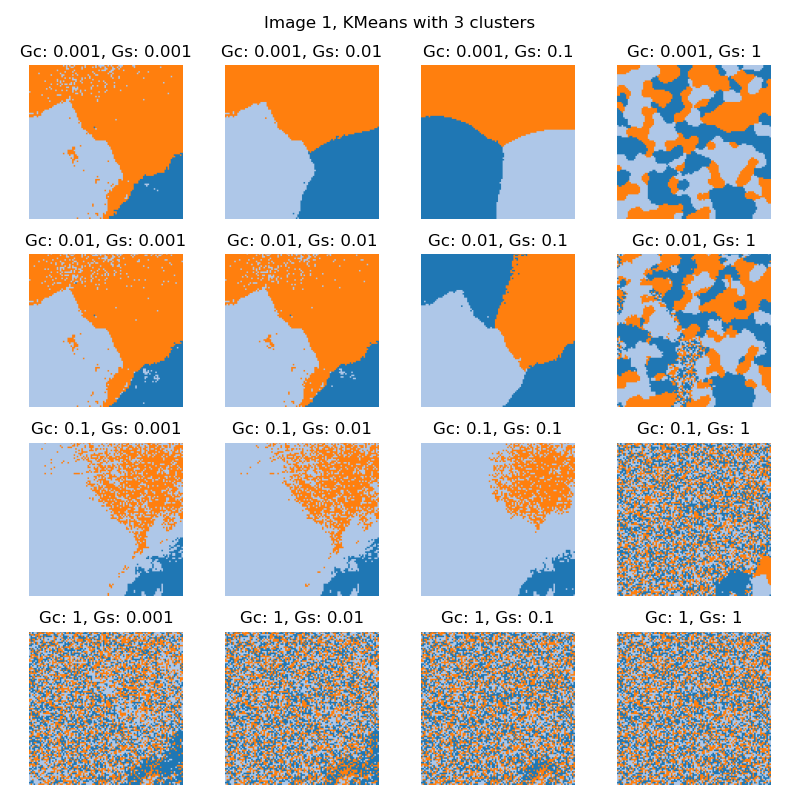
\includegraphics[width=0.5\textwidth]{image1_kmeans-3}
    \caption{The result of gamma values equals 1 are not good.}
\end{figure}

The hyperparameters for the Spectral Clustering(normalized cut and ratio cut) are all the combinations of the following values:

\begin{align*}
\text{n\_clusters} &= [2, 3, 4, 5, 10] \\
\text{gamma\_color} &= [0.0001, 0.005] \\
\text{gamma\_spatial} &= [0.0001, 0.01] \\
\end{align*}

The gamma values for the spectral clustering is based on the kernel K-Means setting of the good gamma values.
I choosed only two gamma values is because the computation time is very long.

\subsubsection{Results \& Discussion}

The original images are:

\begin{figure}[H]
    \centering
    \begin{subfigure}{0.3\textwidth}
        \centering
        
\includegraphics[width=\textwidth]{image1.png}
        \caption{Image 1}
    \end{subfigure}
    \begin{subfigure}{0.3\textwidth}
        \centering
        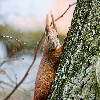
\includegraphics[width=\textwidth]{image2.png}
        \caption{Image 2}
    \end{subfigure}
    \caption{Original Images}
\end{figure}

The file name format for kernel K-Means is:

\texttt{output/image\{i\}\_kmeans-\{init\_method\}-\{n\_clusters\}-\{gamma\_color\}-\{gamma\_spatial\}.gif}

\vspace{1em}

For Spectral Clustering, the file name format is:

\texttt{output/image\{i\}\_sc-\{cut\}-\{init\_method\}-\{n\_clusters\}-\{gamma\_color\}-\{gamma\_spatial\}.gif}

\vspace{1em}

For better visualization, the flat GIFs are restricted up to 10 frames.

\vspace{1em}

Part 1: Clustering \& Visualization

Kernel K-Means:

\begin{figure}[H]
    \centering
    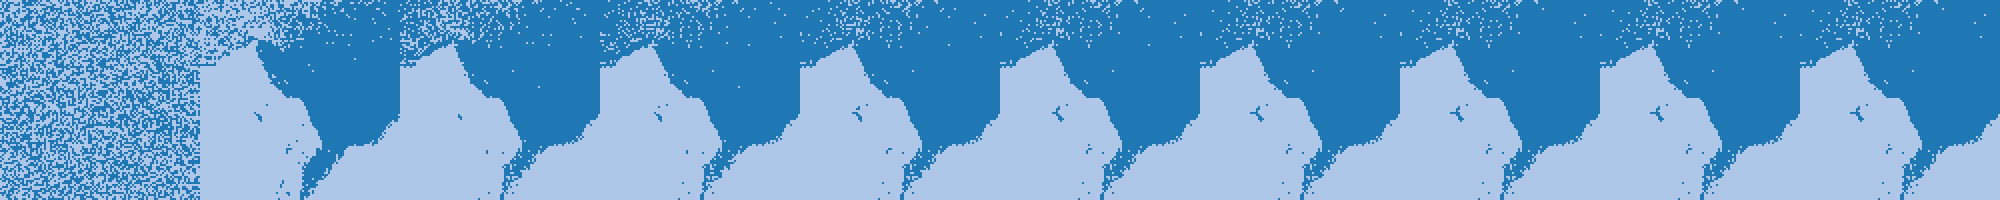
\includegraphics[height=1.6cm]{output_flatgif/flatgif_image1_kmeans-random-2-0.005-0.01.png}
    \caption{output/image1\_kmeans-random-2-0.005-0.01.gif}
\end{figure}

\begin{figure}[H]
    \centering
    
\includegraphics[height=1.6cm]{output_flatgif/flatgif_image2_kmeans-random-2-0.005-0.01.png}
    \caption{output/image2\_kmeans-random-2-0.005-0.01.gif}
\end{figure}

Spectral Clustering with Normalized Cut:

\begin{figure}[H]
    \centering
    
\includegraphics[height=1.6cm]{output_flatgif/flatgif_image1_sc-normalized-random-2-0.005-0.01.png}
    \caption{output/image1\_sc-normalized-random-2-0.005-0.01.gif}
\end{figure}

\begin{figure}[H]
    \centering
    
\includegraphics[height=1.6cm]{output_flatgif/flatgif_image2_sc-normalized-random-2-0.005-0.01.png}
    \caption{output/image2\_sc-normalized-random-2-0.005-0.01.gif}
\end{figure}

Spectral Clustering with Ratio Cut:

\begin{figure}[H]
    \centering
    
\includegraphics[height=1.6cm]{output_flatgif/flatgif_image1_sc-ratio-random-2-0.005-0.01.png}
    \caption{output/image1\_sc-ratio-random-2-0.005-0.01.gif}
\end{figure}

\begin{figure}[H]
    \centering
    
\includegraphics[height=1.6cm]{output_flatgif/flatgif_image2_sc-ratio-random-2-0.005-0.01.png}
    \caption{output/image2\_sc-ratio-random-2-0.005-0.01.gif}
\end{figure}

Discussion: We can see that the Spectral Clustering with Normalized Cut and Ratio Cut have faster convergence than Kernel K-Means. But the result is the same for the 2 clusters setting.

\vspace{1em}

Part2: Try more clusters.

Kernel K-Means:

\begin{figure}[H]
    \centering
    \begin{subfigure}{0.32\textwidth}
        \centering
        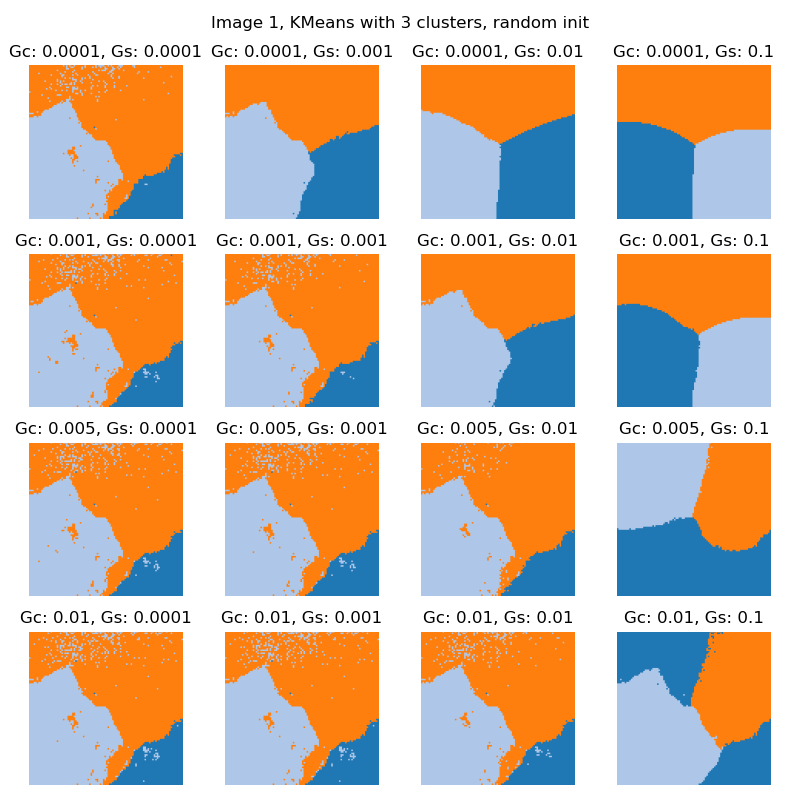
\includegraphics[width=\textwidth]{output_grid/image1_kmeans-random-3.png}
        \caption{3 Clusters}
    \end{subfigure}
    \begin{subfigure}{0.32\textwidth}
        \centering
        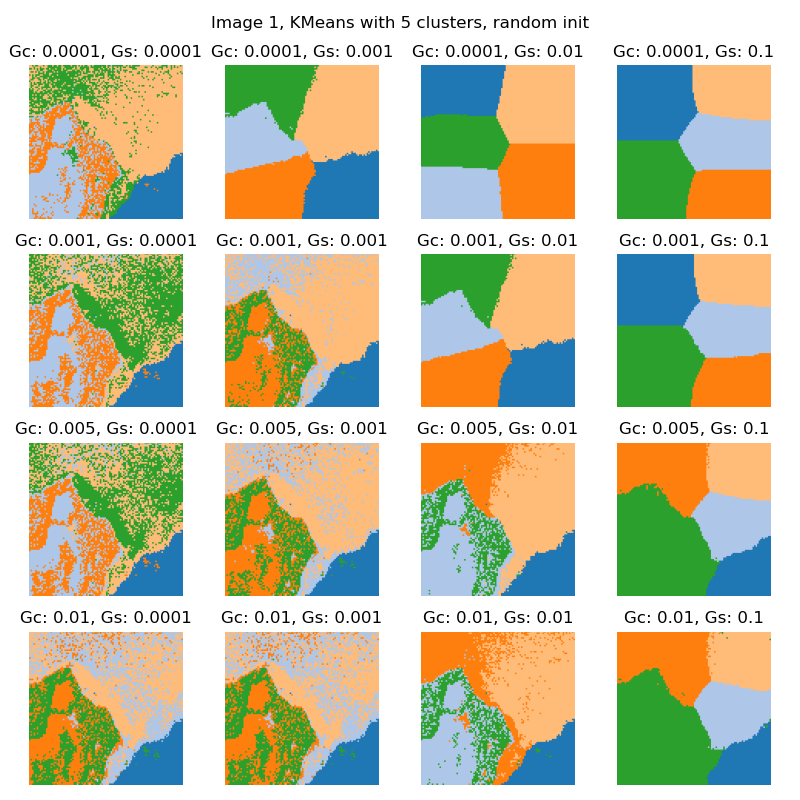
\includegraphics[width=\textwidth]{output_grid/image1_kmeans-random-5.png}
        \caption{5 Clusters}
    \end{subfigure}
    \begin{subfigure}{0.32\textwidth}
        \centering
        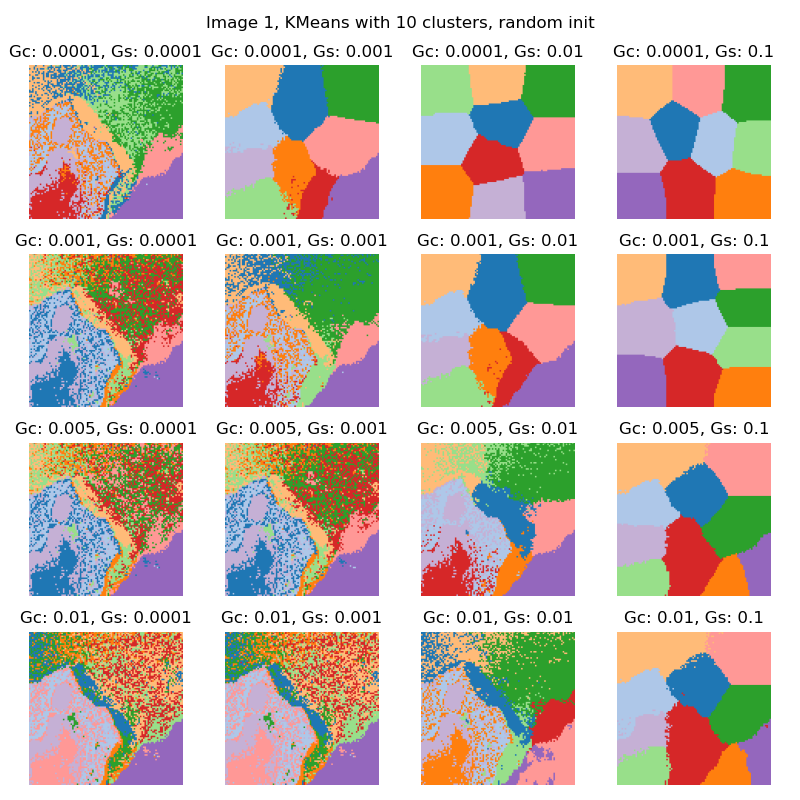
\includegraphics[width=\textwidth]{output_grid/image1_kmeans-random-10.png}
        \caption{10 Clusters}
    \end{subfigure}
    \caption{Kernel K-Means Clustering with Different Number of Clusters (Image 1)}
\end{figure}

\begin{figure}[H]
    \centering
    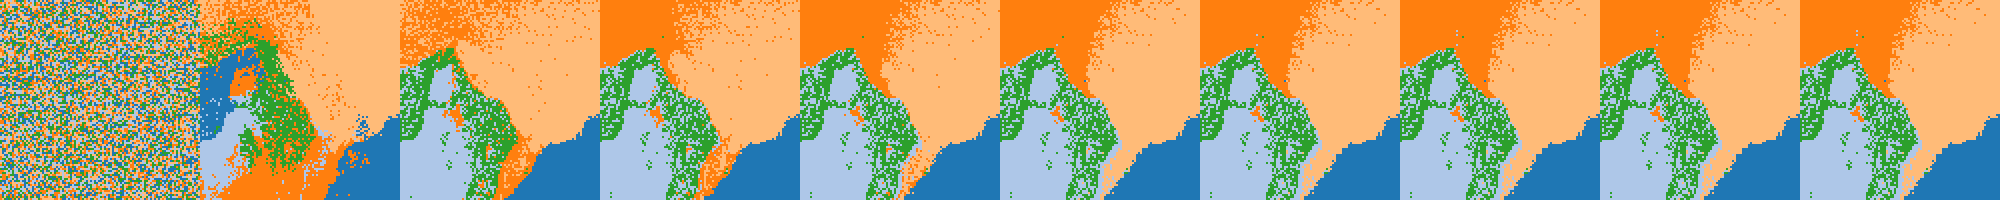
\includegraphics[height=1.6cm]{output_flatgif/flatgif_image1_kmeans-random-5-0.005-0.01.png}
    \caption{output/image1\_kmeans-random-5-0.005-0.01.gif}
\end{figure}

\begin{figure}[H]
    \centering
    \begin{subfigure}{0.32\textwidth}
        \centering
        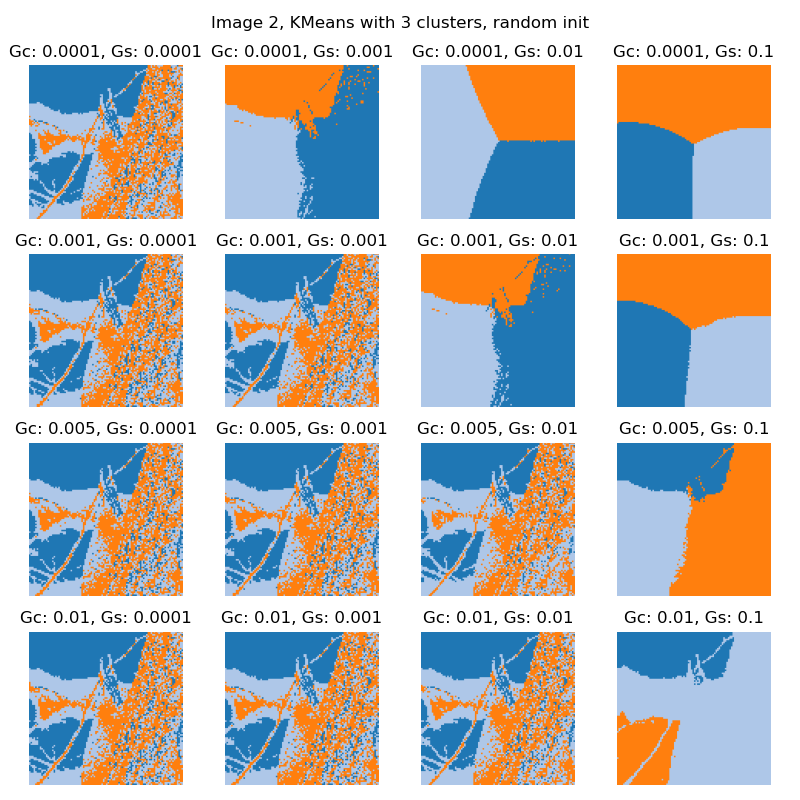
\includegraphics[width=\textwidth]{output_grid/image2_kmeans-random-3.png}
        \caption{3 Clusters}
    \end{subfigure}
    \begin{subfigure}{0.32\textwidth}
        \centering
        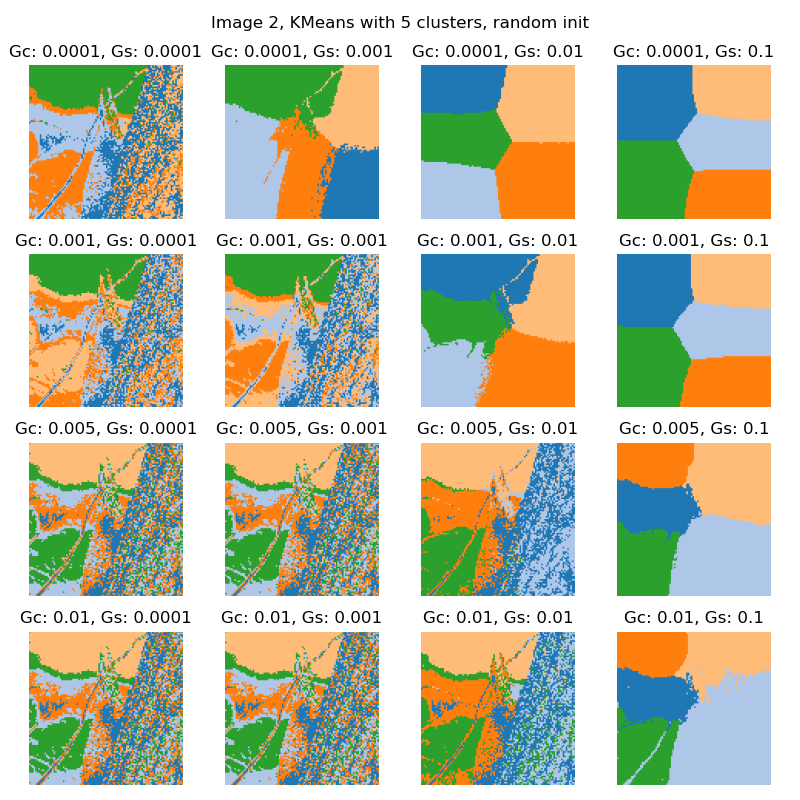
\includegraphics[width=\textwidth]{output_grid/image2_kmeans-random-5.png}
        \caption{5 Clusters}
    \end{subfigure}
    \begin{subfigure}{0.32\textwidth}
        \centering
        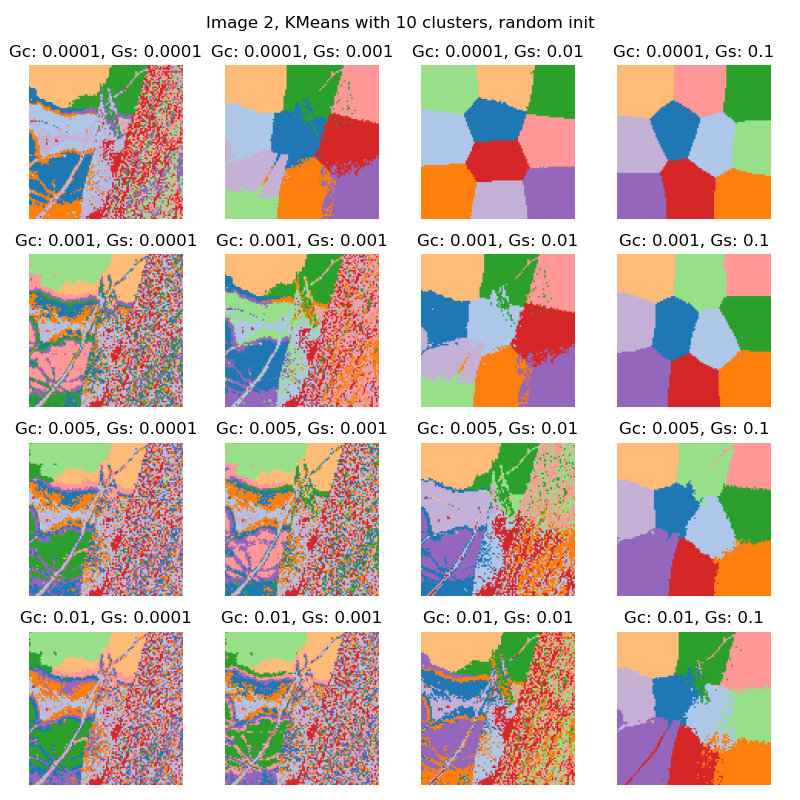
\includegraphics[width=\textwidth]{output_grid/image2_kmeans-random-10.png}
        \caption{10 Clusters}
    \end{subfigure}
    \caption{Kernel K-Means Clustering with Different Number of Clusters (Image 2)}
\end{figure}

\begin{figure}[H]
    \centering
    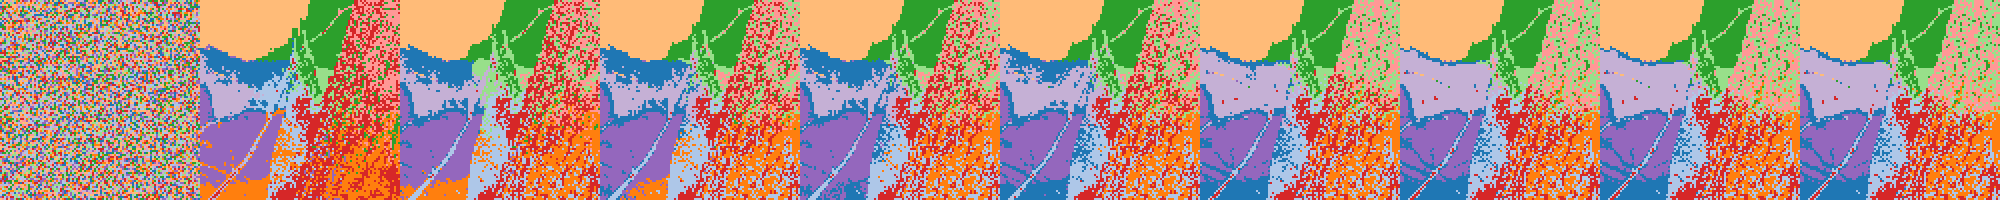
\includegraphics[height=1.6cm]{output_flatgif/flatgif_image2_kmeans-random-10-0.005-0.01.png}
    \caption{output/image2\_kmeans-random-10-0.005-0.01.gif}
\end{figure}

Spectral Clustering with Normalized Cut:

\begin{figure}[H]
    \centering
    \begin{subfigure}{0.32\textwidth}
        \centering
        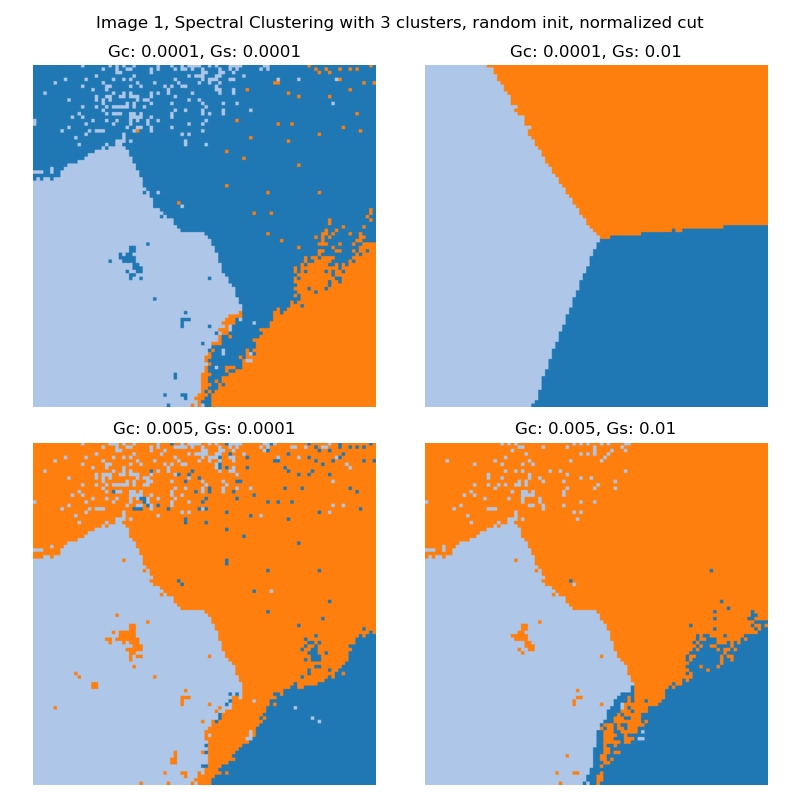
\includegraphics[width=\textwidth]{output_grid/image1_sc-normalized-random-3.png}
        \caption{3 Clusters}
    \end{subfigure}
    \begin{subfigure}{0.32\textwidth}
        \centering
        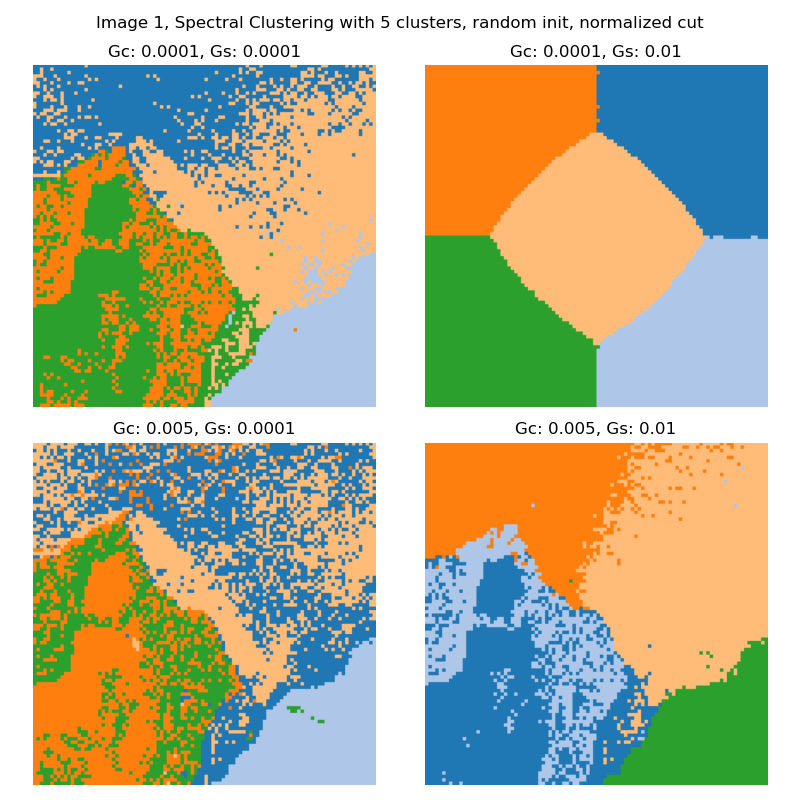
\includegraphics[width=\textwidth]{output_grid/image1_sc-normalized-random-5.png}
        \caption{5 Clusters}
    \end{subfigure}
    \begin{subfigure}{0.32\textwidth}
        \centering
        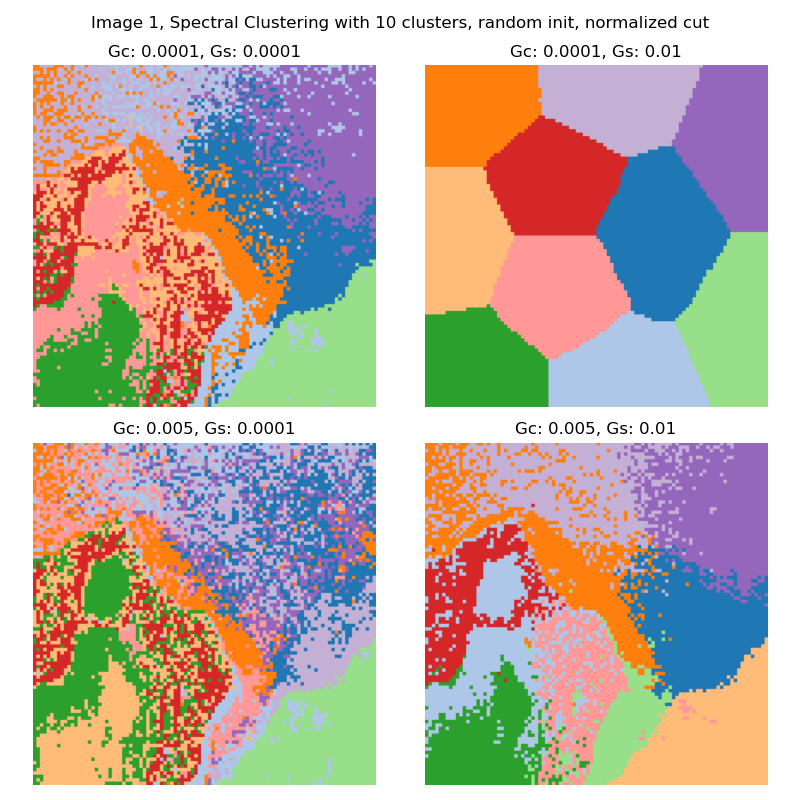
\includegraphics[width=\textwidth]{output_grid/image1_sc-normalized-random-10.png}
        \caption{10 Clusters}
    \end{subfigure}
    \caption{Spectral Clustering with Normalized Cut and Different Number of Clusters (Image 1)}
\end{figure}

\begin{figure}[H]
    \centering
    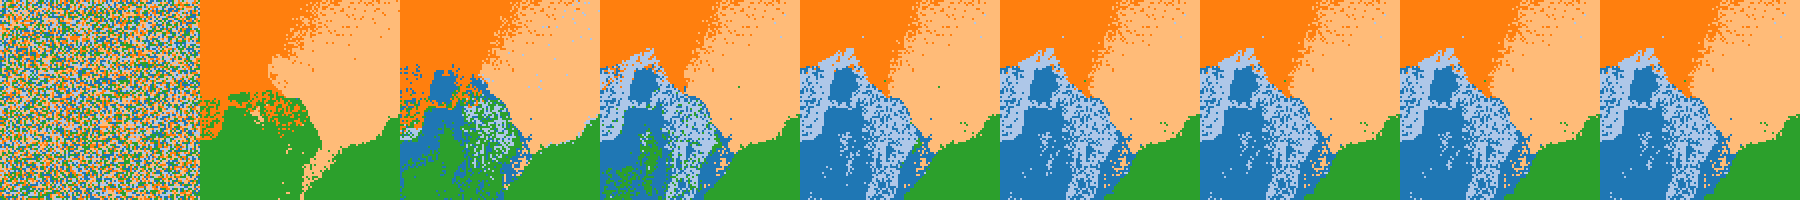
\includegraphics[height=1.6cm]{output_flatgif/flatgif_image1_sc-normalized-random-5-0.005-0.01.png}
    \caption{output/image1\_sc-normalized-random-5-0.005-0.01.gif}
\end{figure}

\begin{figure}[H]
    \centering
    \begin{subfigure}{0.32\textwidth}
        \centering
        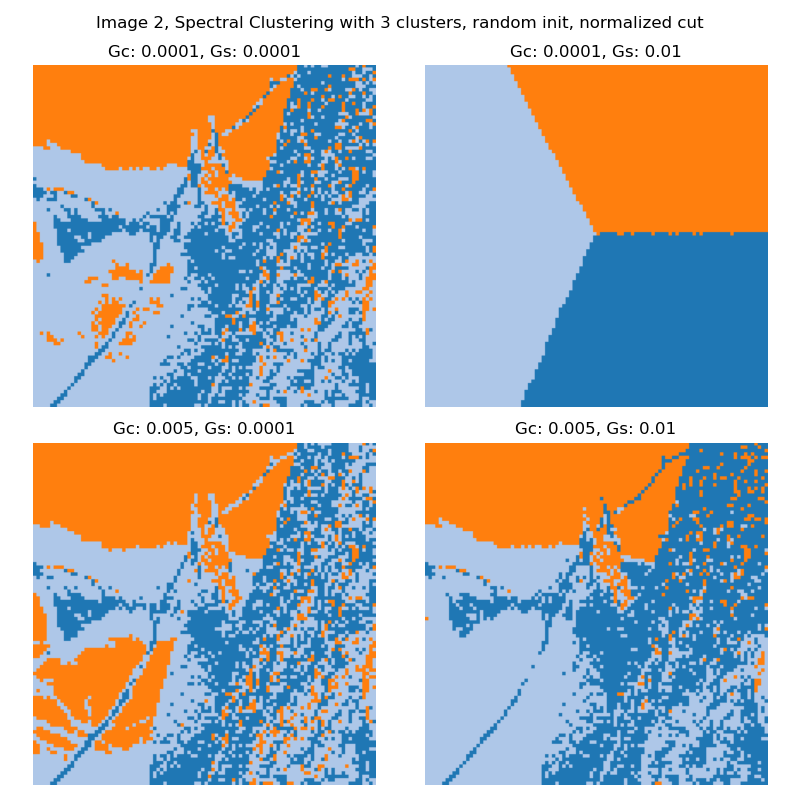
\includegraphics[width=\textwidth]{output_grid/image2_sc-normalized-random-3.png}
        \caption{3 Clusters}
    \end{subfigure}
    \begin{subfigure}{0.32\textwidth}
        \centering
        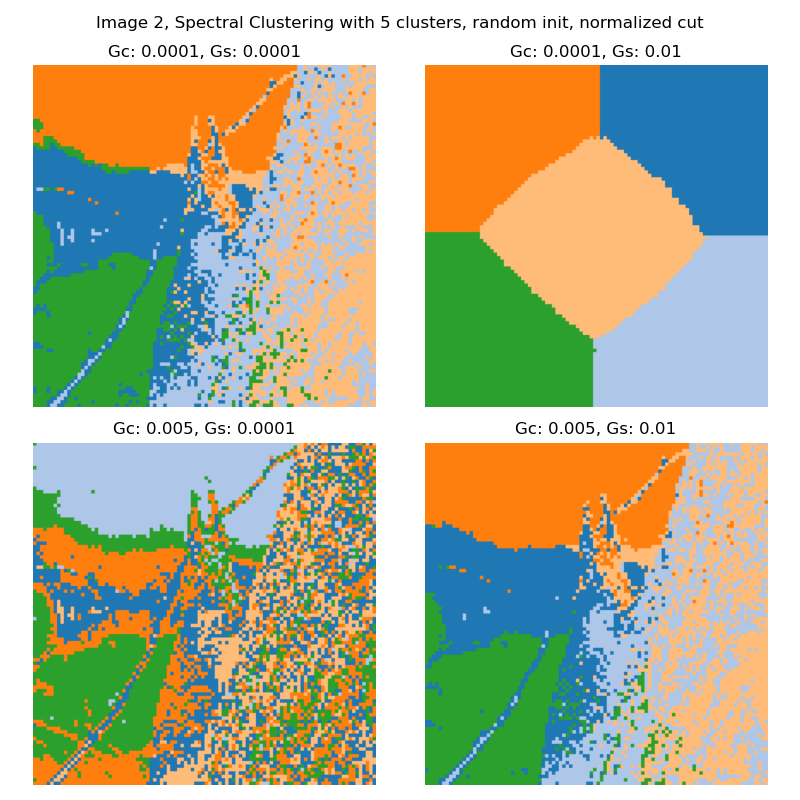
\includegraphics[width=\textwidth]{output_grid/image2_sc-normalized-random-5.png}
        \caption{5 Clusters}
    \end{subfigure}
    \begin{subfigure}{0.32\textwidth}
        \centering
        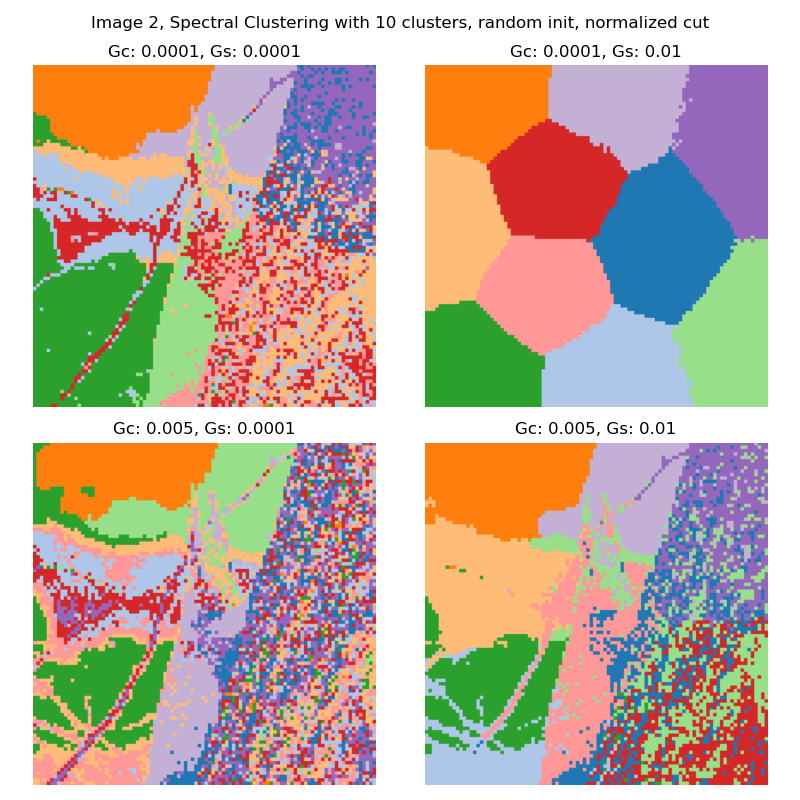
\includegraphics[width=\textwidth]{output_grid/image2_sc-normalized-random-10.png}
        \caption{10 Clusters}
    \end{subfigure}
    \caption{Spectral Clustering with Normalized Cut and Different Number of Clusters (Image 2)}
\end{figure}

\begin{figure}[H]
    \centering
    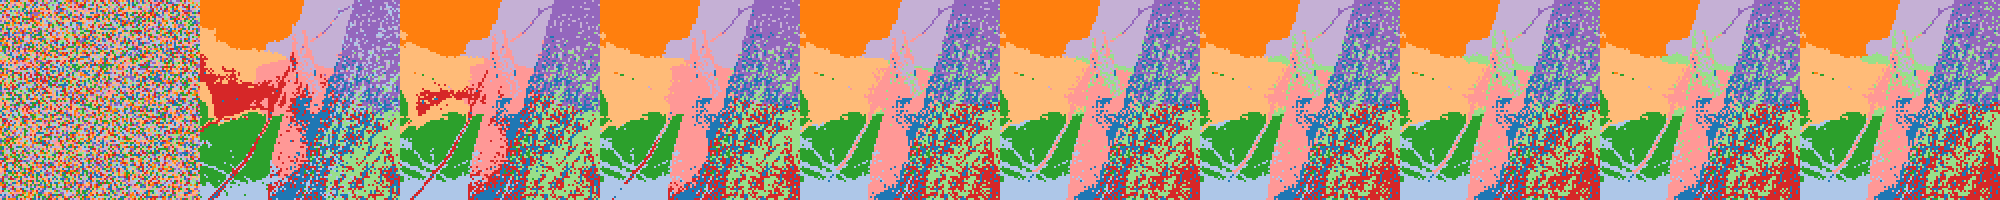
\includegraphics[height=1.6cm]{output_flatgif/flatgif_image2_sc-normalized-random-10-0.005-0.01.png}
    \caption{output/image2\_sc-normalized-random-10-0.005-0.01.gif}
\end{figure}

Spectral Clustering with Ratio Cut:

\begin{figure}[H]
    \centering
    \begin{subfigure}{0.32\textwidth}
        \centering
        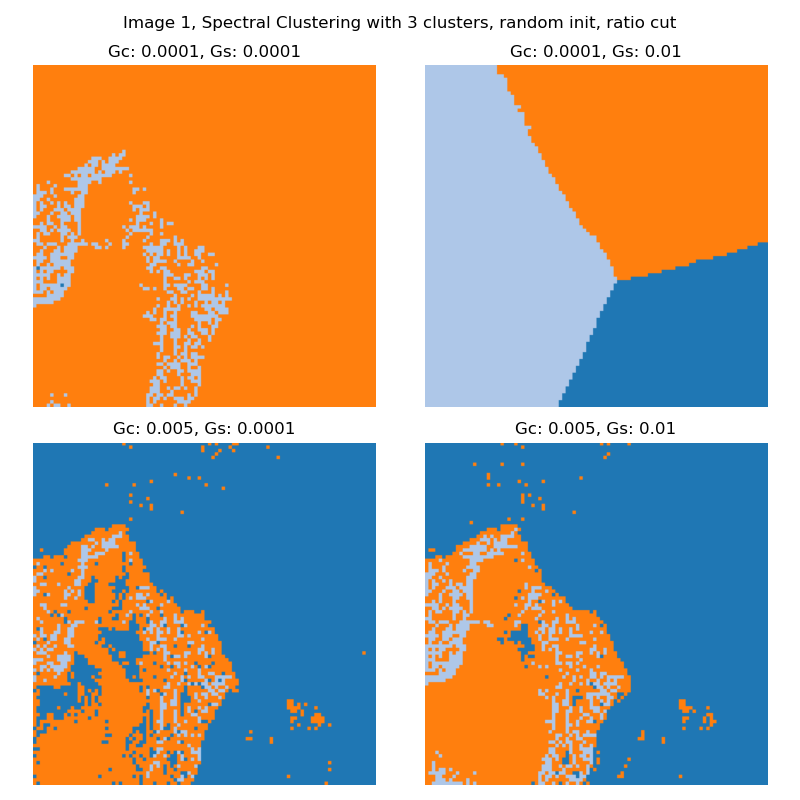
\includegraphics[width=\textwidth]{output_grid/image1_sc-ratio-random-3.png}
        \caption{3 Clusters}
    \end{subfigure}
    \begin{subfigure}{0.32\textwidth}
        \centering
        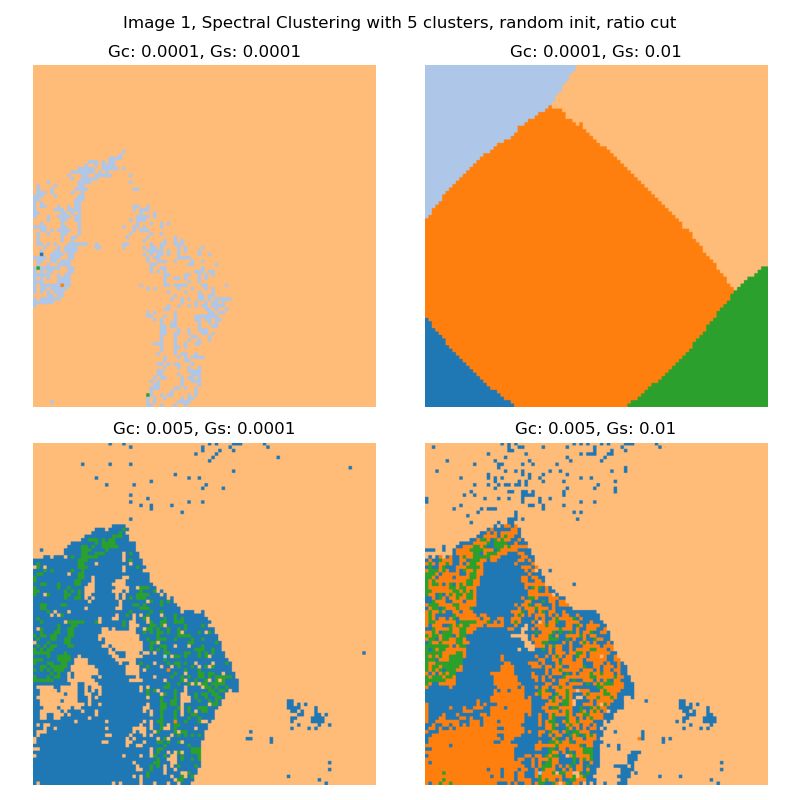
\includegraphics[width=\textwidth]{output_grid/image1_sc-ratio-random-5.png}
        \caption{5 Clusters}
    \end{subfigure}
    \begin{subfigure}{0.32\textwidth}
        \centering
        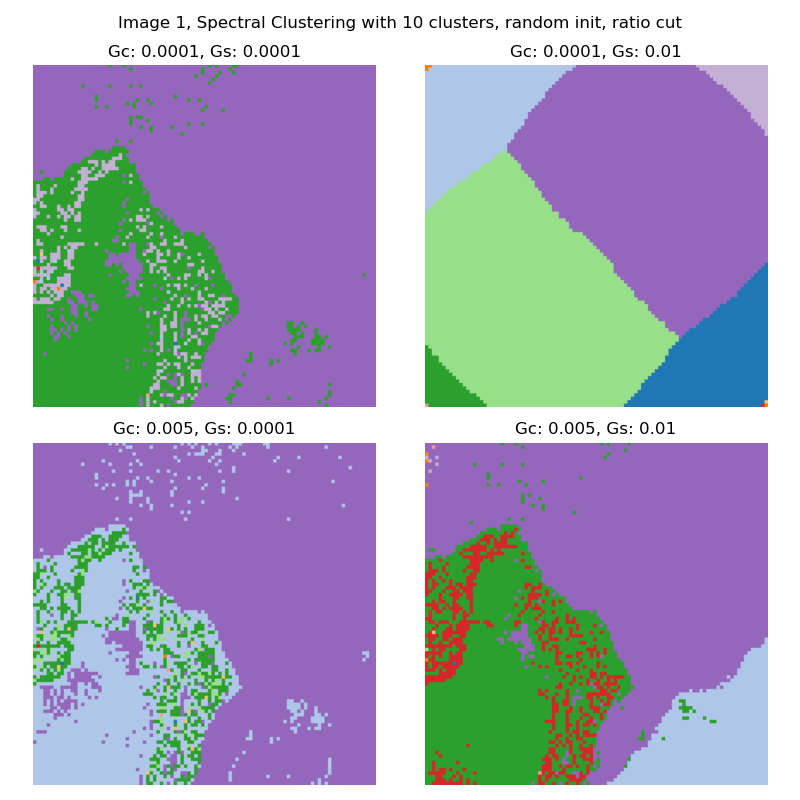
\includegraphics[width=\textwidth]{output_grid/image1_sc-ratio-random-10.png}
        \caption{10 Clusters}
    \end{subfigure}
    \caption{Spectral Clustering with Ratio Cut and Different Number of Clusters (Image 1)}
\end{figure}

\begin{figure}[H]
    \centering
    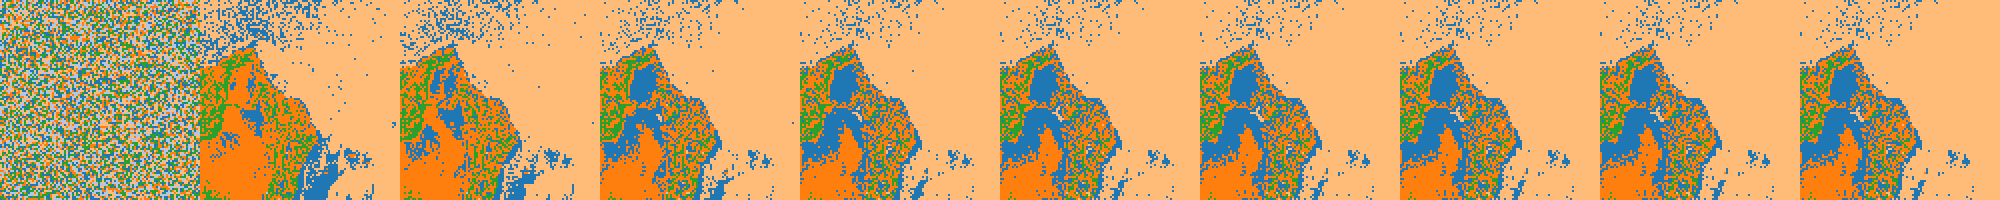
\includegraphics[height=1.6cm]{output_flatgif/flatgif_image1_sc-ratio-random-5-0.005-0.01.png}
    \caption{output/image1\_sc-ratio-random-5-0.005-0.01.gif}
\end{figure}

\begin{figure}[H]
    \centering
    \begin{subfigure}{0.32\textwidth}
        \centering
        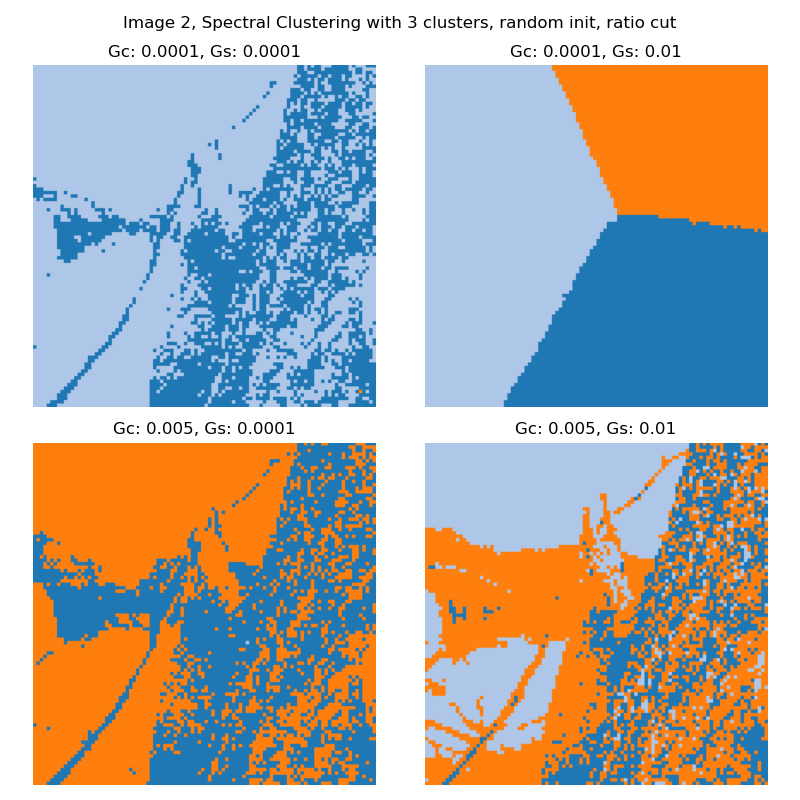
\includegraphics[width=\textwidth]{output_grid/image2_sc-ratio-random-3.png}
        \caption{3 Clusters}
    \end{subfigure}
    \begin{subfigure}{0.32\textwidth}
        \centering
        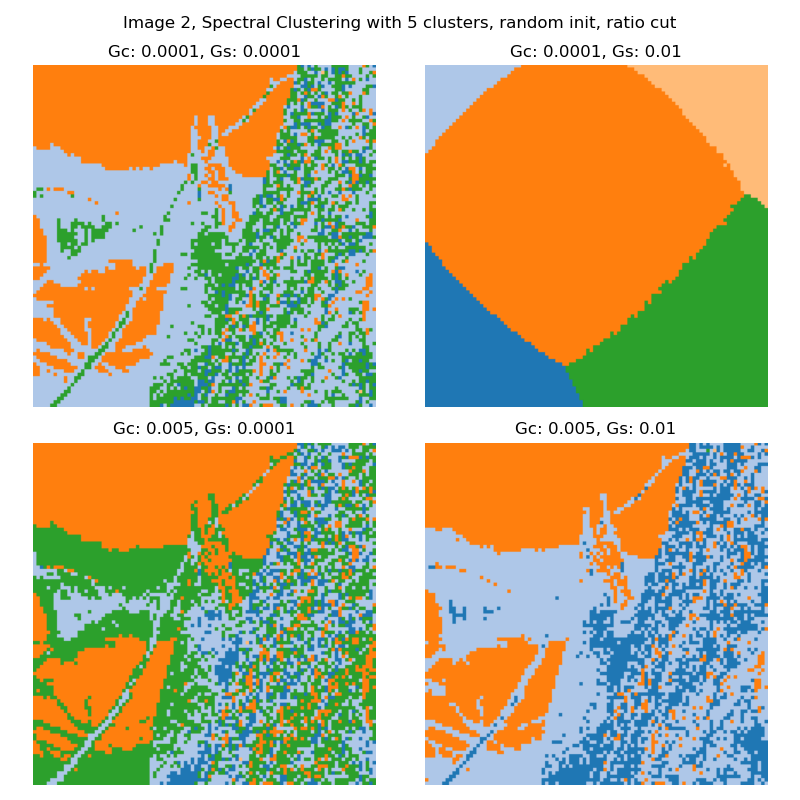
\includegraphics[width=\textwidth]{output_grid/image2_sc-ratio-random-5.png}
        \caption{5 Clusters}
    \end{subfigure}
    \begin{subfigure}{0.32\textwidth}
        \centering
        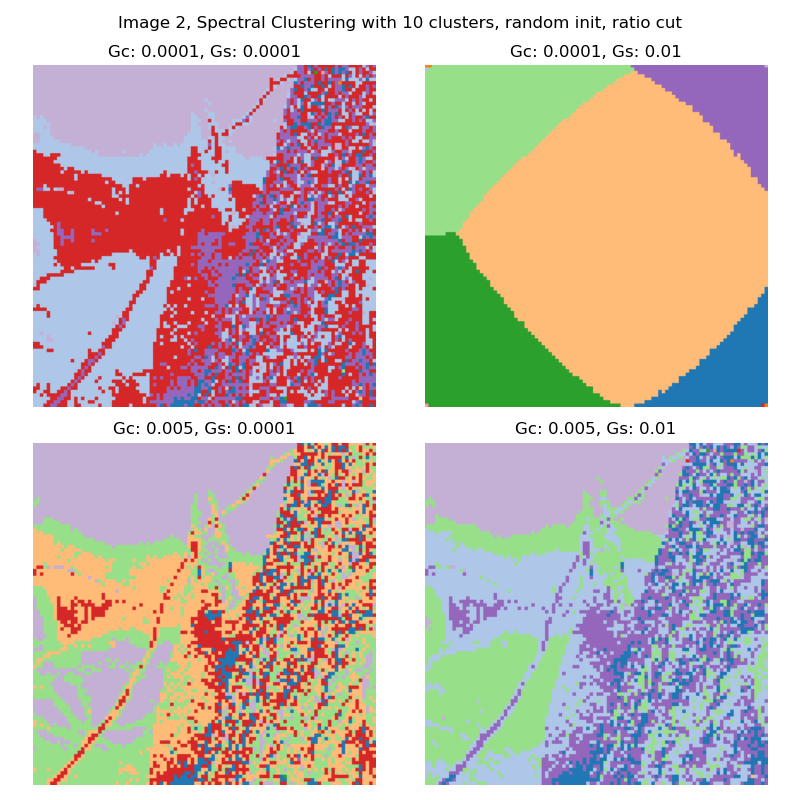
\includegraphics[width=\textwidth]{output_grid/image2_sc-ratio-random-10.png}
        \caption{10 Clusters}
    \end{subfigure}
    \caption{Spectral Clustering with Ratio Cut and Different Number of Clusters (Image 2)}
\end{figure}

\begin{figure}[H]
    \centering
    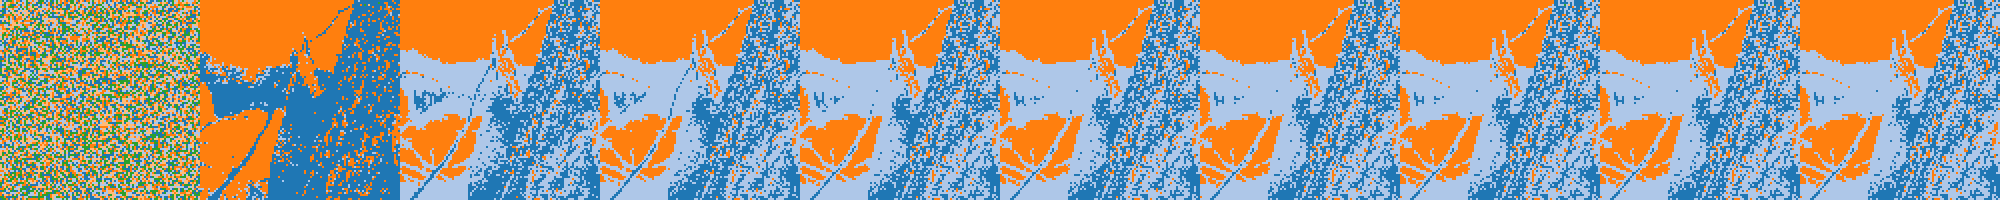
\includegraphics[height=1.6cm]{output_flatgif/flatgif_image2_sc-ratio-random-5-0.005-0.01.png}
    \caption{output/image2\_sc-ratio-random-5-0.005-0.01.gif}
\end{figure}

Discussion: We can see that for different image, the best number of clusters is different. For image 1, 5 clusters is the best, but for image 2, 10 clusters is the best in my opinion.

\vspace{1em}

Part3: Try different initializations.

Compare random and kmeans++ initialization methods.

Kernel K-Means:

\begin{figure}[H]
    \centering
    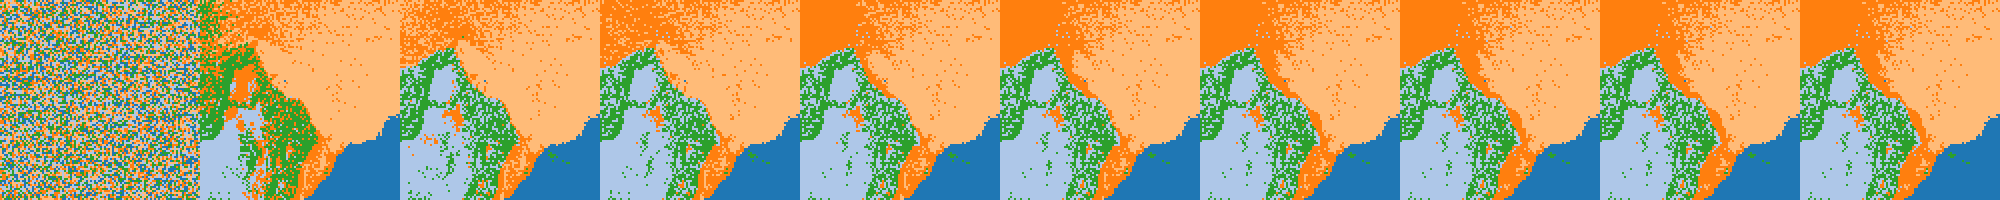
\includegraphics[height=1.6cm]{output_flatgif/flatgif_image1_kmeans-random-5-0.01-0.01.png}
    \caption{output/image1\_kmeans-random-5-0.01-0.01.gif}
\end{figure}

\begin{figure}[H]
    \centering
    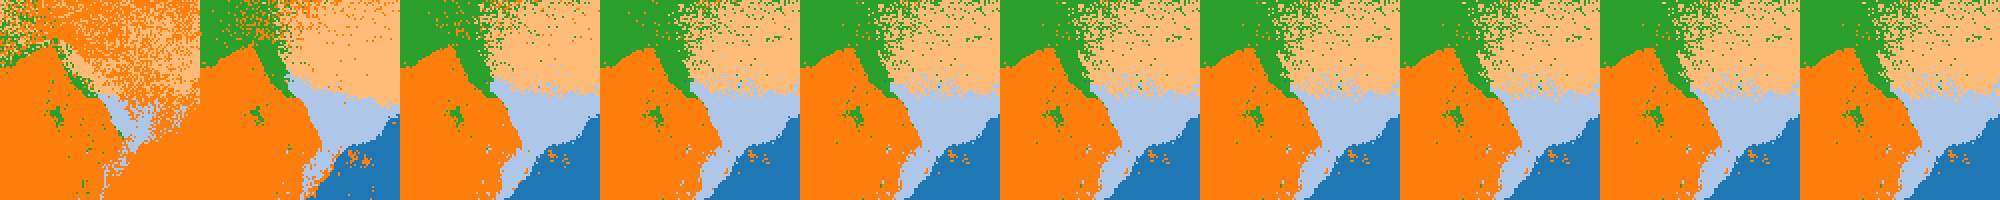
\includegraphics[height=1.6cm]{output_flatgif/flatgif_image1_kmeans-kmeans++-5-0.01-0.01.png}
    \caption{output/image1\_kmeans-kmeans++-5-0.01-0.01.gif}
\end{figure}

Spectral Clustering with Normalized Cut:

\begin{figure}[H]
    \centering
    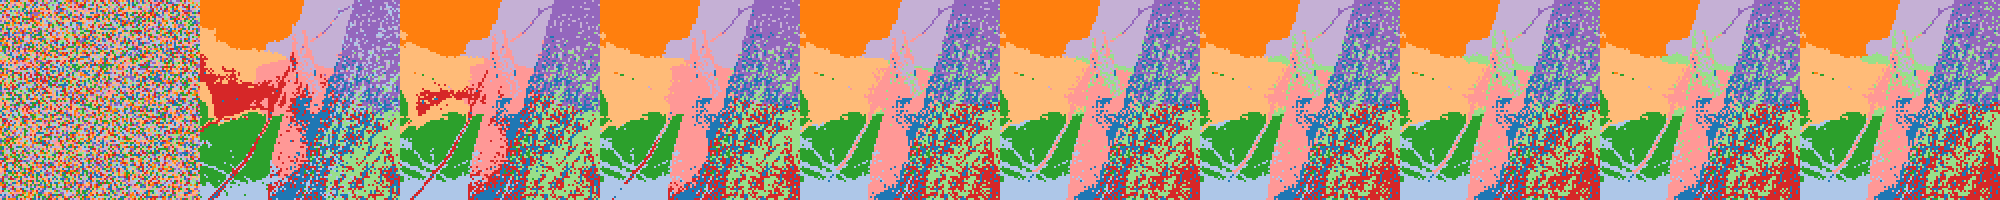
\includegraphics[height=1.6cm]{output_flatgif/flatgif_image2_sc-normalized-random-10-0.005-0.01.png}
    \caption{output/image2\_sc-normalized-random-10-0.005-0.01.gif}
\end{figure}

\begin{figure}[H]
    \centering
    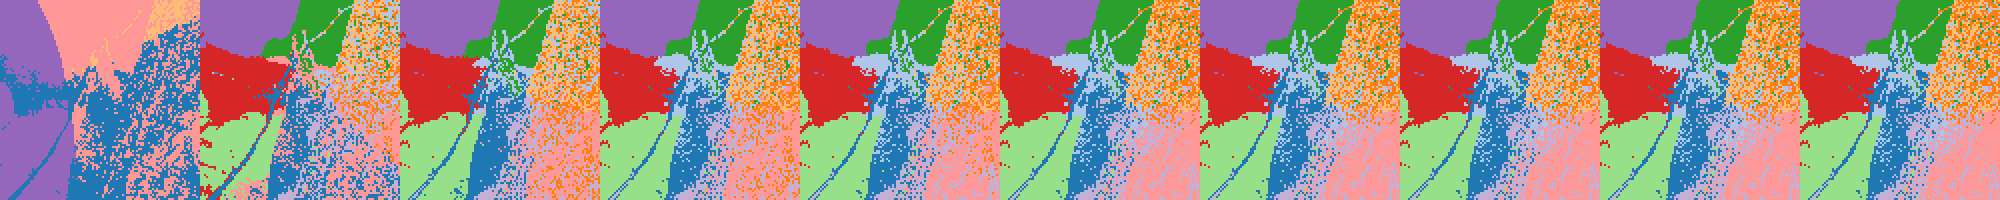
\includegraphics[height=1.6cm]{output_flatgif/flatgif_image2_sc-normalized-kmeans++-10-0.005-0.01.png}
    \caption{output/image2\_sc-normalized-kmeans++-10-0.005-0.01.gif}
\end{figure}

Spectral Clustering with Ratio Cut:

\begin{figure}[H]
    \centering
    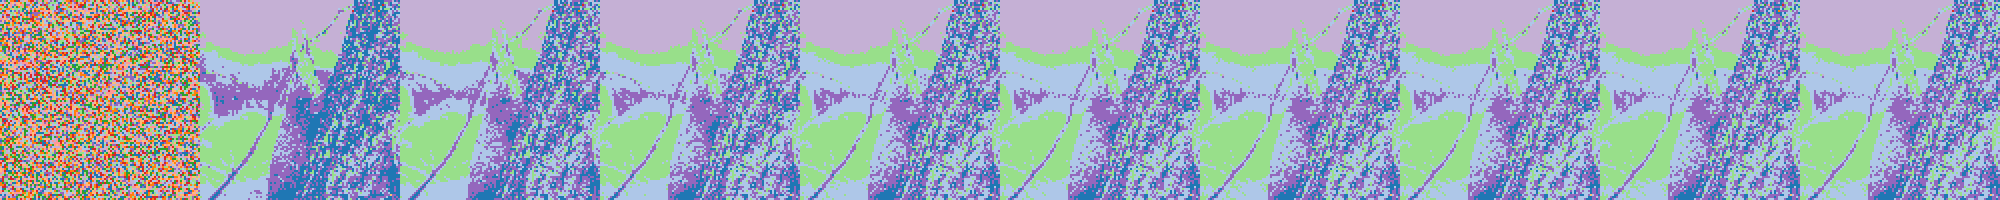
\includegraphics[height=1.6cm]{output_flatgif/flatgif_image2_sc-ratio-random-10-0.005-0.01.png}
    \caption{output/image2\_sc-normalized-random-10-0.005-0.01.gif}
\end{figure}

\begin{figure}[H]
    \centering
    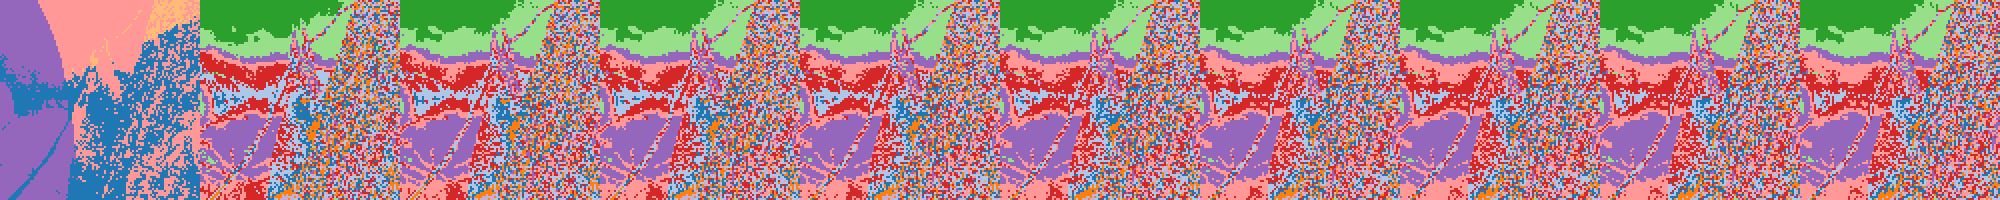
\includegraphics[height=1.6cm]{output_flatgif/flatgif_image2_sc-ratio-kmeans++-10-0.005-0.01.png}
    \caption{output/image2\_sc-normalized-kmeans++-10-0.005-0.01.gif}
\end{figure}

Discussion: We can see that the kmeans++ initialization method is often better than the random initialization method in terms of final results. But for \texttt{image2\_sc-normalized-10-0.005-0.01} setting, the random initialization method can split the background branches, but the kmeans++ initialization method cannot.

\vspace{1em}

Part4: Experiments on the coordinates in the eigenspace.

I've tried different examination results for the clusters. For illustration, I'll only show one setting:

\texttt{image1\_sc-normalized-random-5-0.005-0.01}

\begin{figure}[H]
    \centering
    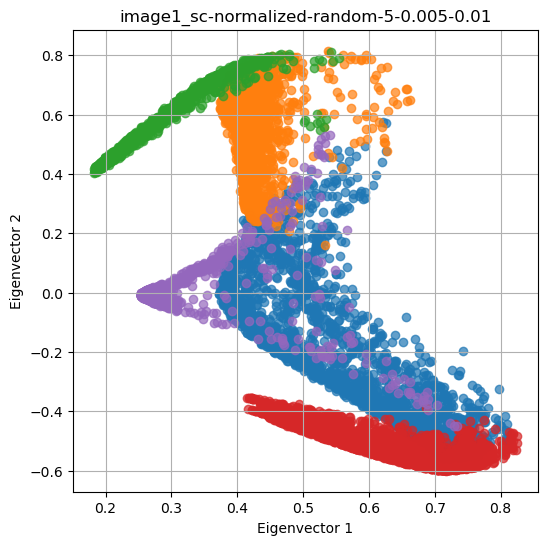
\includegraphics[width=0.5\textwidth]{image1_sc-normalized-random-5-0.005-0.01.png}
    \caption{Eigenspace Clustering Results}
\end{figure}

\begin{lstlisting}
Cluster 0
Max Distance to Centroid: 0.8495459656969779
Avg Distance to Centroid: 0.45561859167587093
Variance: [0.00702723 0.06229196 0.03387403 0.08425219 0.0488355 ]

Cluster 1
Max Distance to Centroid: 0.8481972031426014
Avg Distance to Centroid: 0.3535578822908737
Variance: [0.00902073 0.01368432 0.01549015 0.04152903 0.06668715]

Cluster 2
Max Distance to Centroid: 0.8602263446479639
Avg Distance to Centroid: 0.36227211835339174
Variance: [0.01424316 0.04900694 0.00791408 0.05496922 0.03016205]

Cluster 3
Max Distance to Centroid: 0.8339250191234534
Avg Distance to Centroid: 0.38807671155852674
Variance: [0.00721068 0.00574738 0.04644279 0.04185334 0.07261933]

Cluster 4
Max Distance to Centroid: 0.8861002049928656
Avg Distance to Centroid: 0.1689602870193146
Variance: [0.00681353 0.01050571 0.00362991 0.01246515 0.01890811]
\end{lstlisting}

Discussion: We can see that the points in the eigenspace are clustered well.

\subsection{Observations and Discussions}

\subsubsection{Compare the performance between different clustering methods.}

Kernel K-Means and Spectral Clustering show similar performance, but Spectral Clustering converges faster in some settings, particularly with Normalized Cut, providing more stable clustering results.

\subsubsection{Compare the execution time of different settings.}

Kernel K-Means generally completes within 10 to 30 seconds. However, for higher cluster counts or cases where convergence is challenging, the runtime increases significantly. Spectral Clustering, on the other hand, requires approximately 2 minutes to compute eigenvalues and eigenvectors. Since this calculation only depends on the cut method and gamma values, the eigen results can be cached, enabling subsequent clustering with different cluster counts and initialization methods to complete within seconds.

\subsubsection{Anything you want to discuss.}

For higher-dimensional data, Spectral Clustering may perform better. Future work could focus on improving computational efficiency or exploring other methods suitable for non-linear data distributions.

\end{document}